\documentclass[a4paper,10pt, twocolumn]{article}

%Packages
\usepackage{graphicx}
\usepackage{listings}
\usepackage[utf8x]{inputenc} %accenti in Linux
\usepackage{amsmath}
\usepackage{amsfonts}
\usepackage{amssymb}
%\usepackage[latin1]{inputenc} %accenti in Windows

%Commands
\newcommand{\Fig}[1]{Fig.~\ref{#1}}
\newcommand{\Tab}[1]{Table~\ref{#1}}
\newcommand{\annex}{Annex}
\newcommand{\tab}{Table}
\newcommand{\sect}{Section}
\newcommand{\scode}[1]{\texttt{#1}} %In-line code

% Title Page
\title{math-parser}
\author{Riccardo Manfrin \\ \{namesurnameatthemostpopularemailaccountproviderdotcom\}}

% \begin{figure}[htbp]
%   \centering
%   \includegraphics[scale=0.40]{pics/fig00.png}
%   \caption{Device architecture}\label{fig:02:name}
% \end{figure}

% \begin{table*}[htbp]
% \centering
% \scriptsize
%  \begin{tabular}{|c|c|l|}
%  \hline
%  \end{tabular}
%  \small
%  \caption{cap}\label{table:xxx:label}
% \end{table*}



\lstset{
	frame=tb,	%Possible attributes : single,TB,tb,lrtb,LRTB
	basicstyle=\scriptsize,
	%columns=fullflexible,
	fontadjust=true,
	commentstyle=\itshape,
	language=c,
	breaklines=true,
}

\begin{document}
\maketitle
\begin{abstract}
This is a short documentation to explain how to realize a runtime math parser library in C.
In order to produce a flexible parser it is important to grant it the required flexibility. In particular we want our parser to handle any new operator's definitions.
The guide will try to give a practical approach based on personal experience to develop such parser.
\end{abstract}
\section{Identifying support data structures}

Considering that every mathematical operation is made by at most 2 operands and 1 operator, we have that the best suited support data structure for this kind of task is a binary tree.

We note that the parser algorithm can be splitted in 2 sub tasks: 
\begin{itemize}
 \item Generating the binary tree from the mathematical expression
 \item Calculating the result of the expression from the binary tree.
\end{itemize}

\subsection{Generating the Binary Tree}
This task can be performed in a recursive fashion. We first need to identify the type of operations we want to allow: we distinguish between 2-operands (2o) operations and 1-operand (1o) operations, as shown in \Tab{table:000:optypes}.

\begin{table}[htbp]
\centering
\scriptsize
 \begin{tabular}{|l l|c|}
 \hline
 	& OPERATION TYPES & \# OPERANDS \\
 \hline
 	$ (a + b)$ & $\rightarrow c | \mathbb{R}^2 \rightarrow \mathbb{R}$ & 2 \\
 	$ (a - b)$ & $\rightarrow c | \mathbb{R}^2 \rightarrow \mathbb{R}$ & 2 \\
 	$ (a * b)$ & $\rightarrow c | \mathbb{R}^2 \rightarrow \mathbb{R}$ & 2 \\
 	$ (a / b)$ & $\rightarrow c | \mathbb{R}^2 \rightarrow \mathbb{R}$ & 2 \\
 	$ (a \;\hat{}\; b)$ & $\rightarrow c | \mathbb{R}^2 \rightarrow \mathbb{R}$ & 2 \\
 	$ log10(a)$ & $\rightarrow b | \mathbb{R} \rightarrow \mathbb{R}$ & 1 \\
 	$ log2(a)$ & $\rightarrow b | \mathbb{R} \rightarrow \mathbb{R}$ & 1 \\
 	$ sin(a)$ & $\rightarrow b | \mathbb{R} \rightarrow \mathbb{R}$ & 1 \\
 	$ cos(a)$ & $\rightarrow b | \mathbb{R} \rightarrow \mathbb{R}$ & 1 \\
 	$ tan(a)$ & $\rightarrow b | \mathbb{R} \rightarrow \mathbb{R}$ & 1 \\
 	$ ctan(a)$ & $\rightarrow b | \mathbb{R} \rightarrow \mathbb{R}$ & 1 \\
 	$ exp(a)$ & $\rightarrow b | \mathbb{R} \rightarrow \mathbb{R}$ & 1 \\
 	$ a$ & $\rightarrow a | \mathbb{R} \rightarrow \mathbb{R}$ & 1 \\
 \hline
 \end{tabular}
 \small
 \caption{Operation types}\label{table:000:optypes}
\end{table}

Let's start from a simple observation about the generated binary tree from the mathematical expression: whether the tree is balanced or not we don't have an efficiency loss as we anyway have to run our solver algorithm throughout every node (operation) of the tree.

Another important observation is that if we proceed with an ``inorder'' algorithm to expand the tree, we will need to process every node just once. In facts, when we enter a node (starting from the root), we check the first highest priority operation available in the expression outside the most external brackets and expand it. Once the procedure is over we find ourself to be inside the root of a new subtree whose the inner nodes are operations to be calculated, while the leaf nodes are expression to be expanded again.
 
There's another thing to note about the outcome of an expanding procedure: when we deal with 2o operations (highest priority), we can encounter multiple instances of them in a single node, to be handled. Once we have processed all of 2o operations outside the brackets, we start processing nodes that should have at most 1o operations. As we know that these operations require brackets to specify the operand, and we already got rid of the 2o operations, there will be at most one single instance of such operations per node.

The approach we follow to create the b-tree starts from taking the mathematical expression and putting it into the root of the BTree.





\subsection{Calculating the result}

\begin{itemize}
 \item assigning variables name a numeric value,
 \item recursively compute every ``operator-leaf'' operation in a post-order fashion.
\end{itemize}

\newpage

\section{Annex}\label{Annex}
\begin{figure*}[htb]
 \centering
 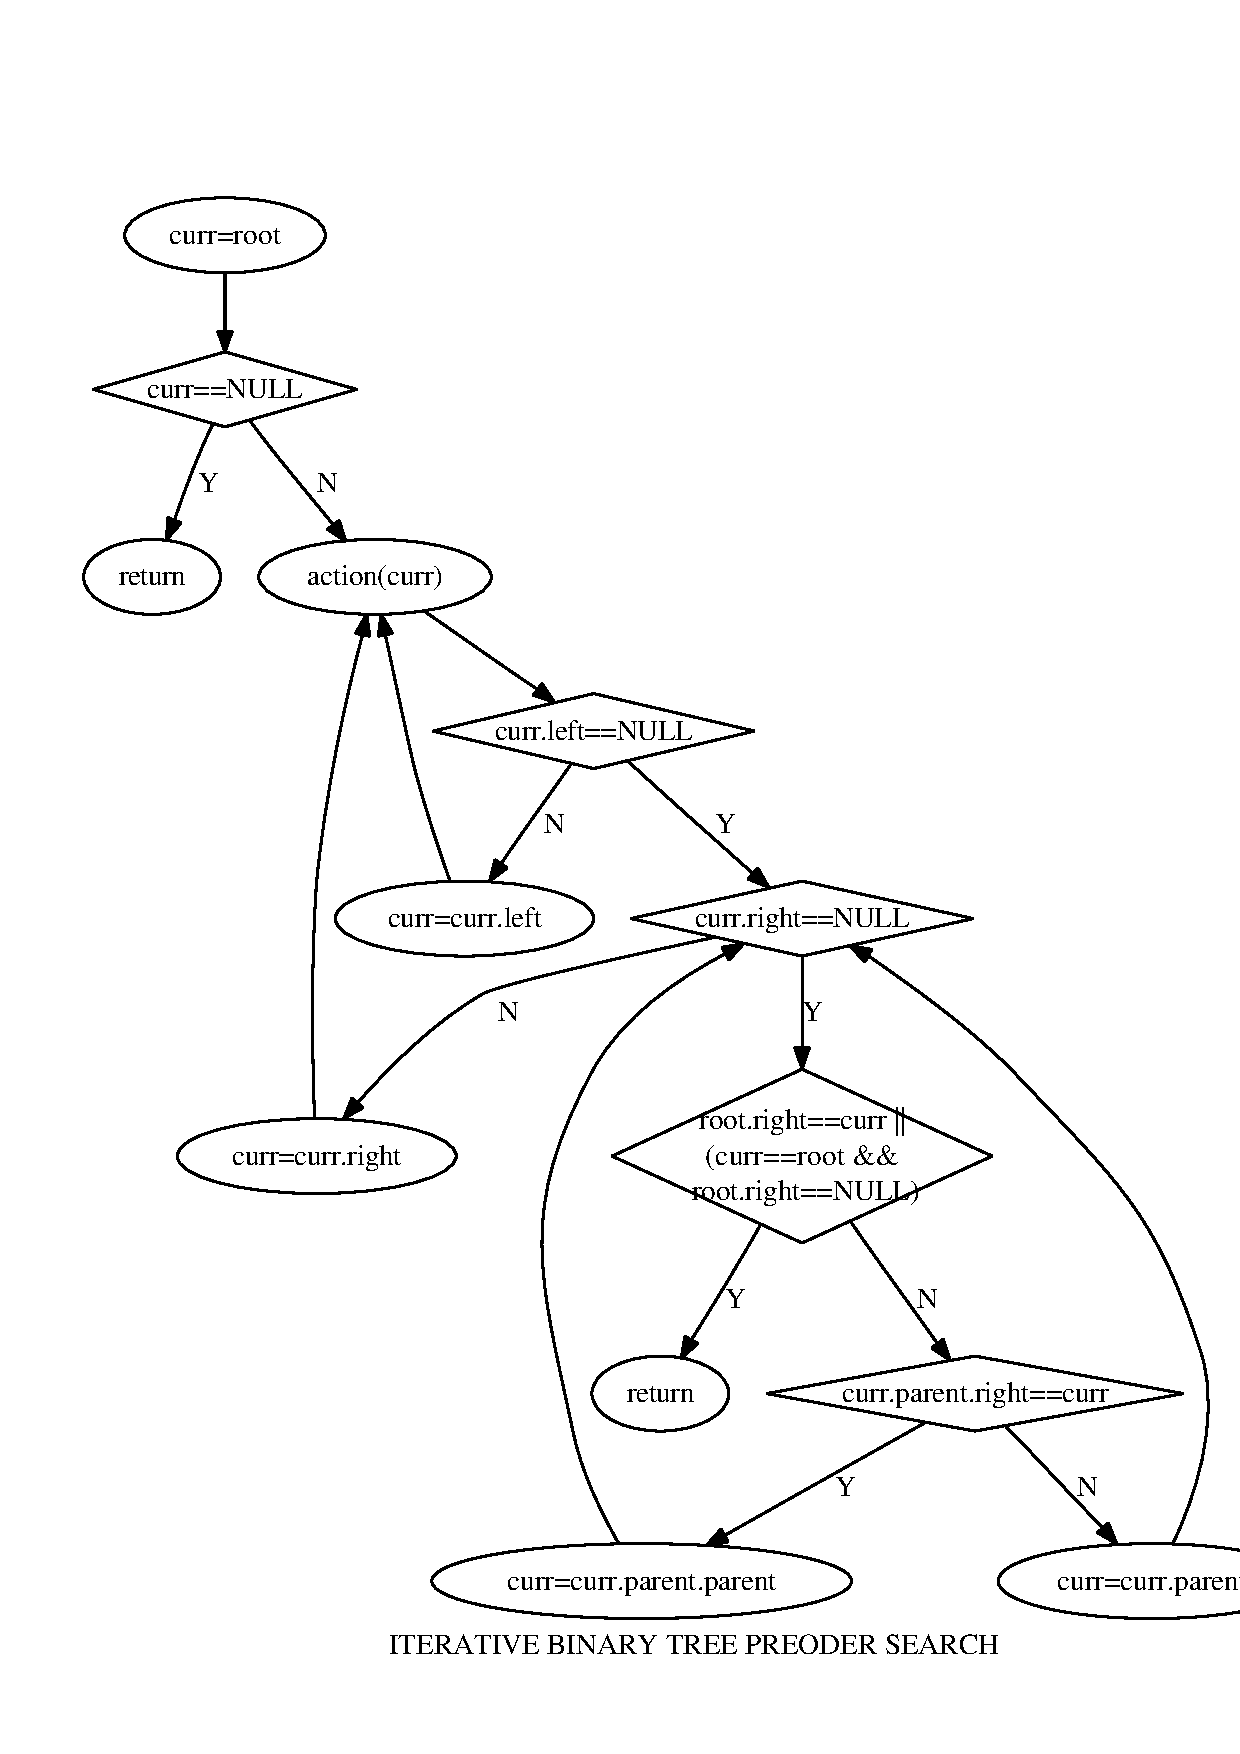
\includegraphics[width=0.8\textwidth]{pics/img003}
 \caption{Inorder iterative algorithm}
 \label{fig:05:001:Inorder_iterative}
\end{figure*}

\begin{figure*}[htb]
 \centering
 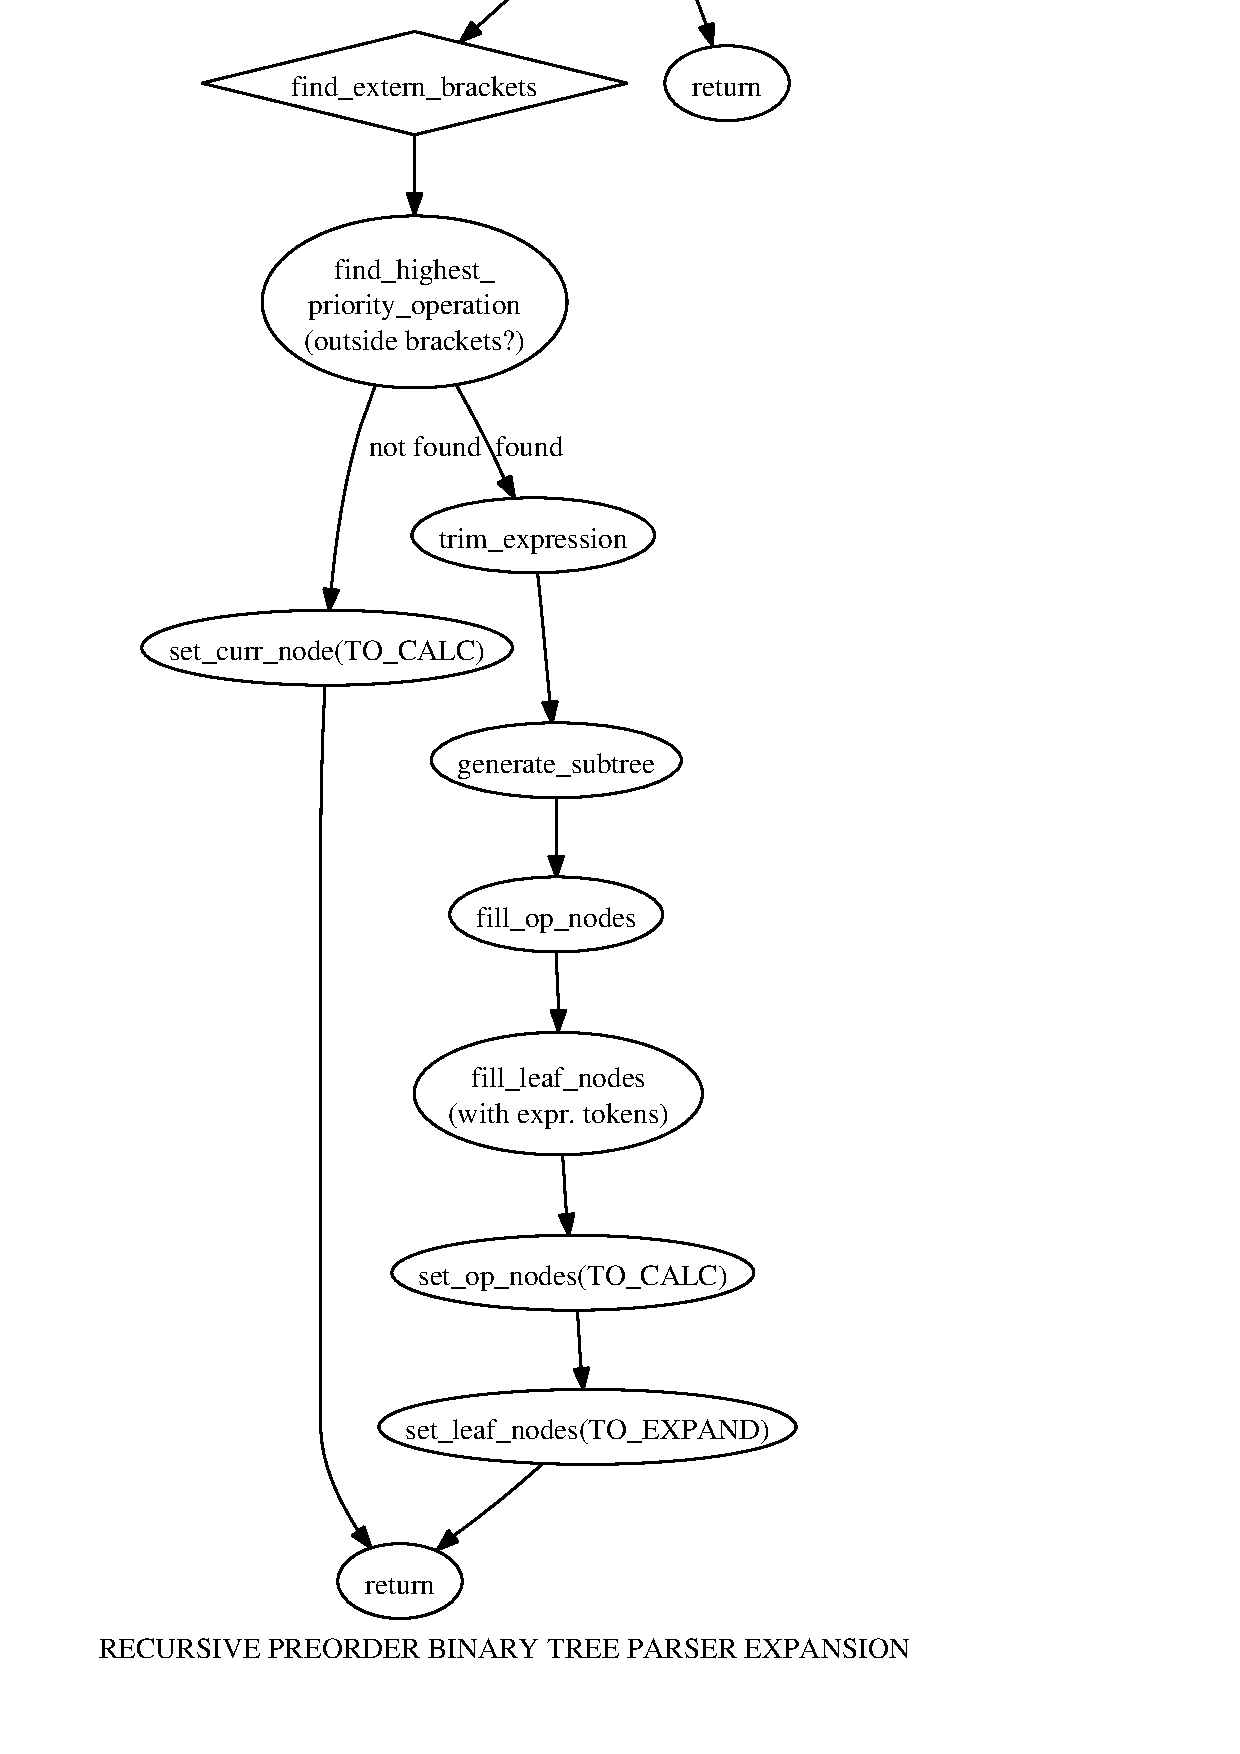
\includegraphics[width=0.5\textwidth]{pics/img004}
 \caption{Node expanding algorithm (for recursive usage)}
 \label{fig:05:004:Node Expanding}
\end{figure*}

%\begin{lstlisting}

%\end{lstlisting}

\end{document}

